% Koma class
\documentclass[a4paper, oneside]{scrartcl}   

\usepackage{a4wide}

%------------------
% language = english
\usepackage[english, german]{babel}	% Umlaute mit \"u
\usepackage[latin1]{inputenc}
\usepackage{enumitem}

% margins + Kopf- und Fusszeilen
\usepackage[left = 2.5cm, right = 2.5cm, top = 2cm, bottom = 3cm]{geometry}
\usepackage{scrpage2} 
\pagestyle{scrheadings}
\clearscrheadfoot
\rehead{\headmark}
\lehead{\pagemark}
\lohead{\headmark}
\rohead{\pagemark} 

% math
\usepackage{amssymb}
\usepackage{amsmath}

% figures
\usepackage{tikz}
\usepackage{graphicx}

% section-Zaehler wird neu gesetzt:
\setcounter{section}{11}
%------------------
\author{Sascha Meiers, Martin Seeger}
\title{Exercise 11, Discrete Mathematics for Bioinformatics}
\date{Winter term 2011/2012}


\begin{document}
\maketitle

%---------------------------------------------------------------------------------------------------

\subsection{Lagrangean Relaxation I}

\renewcommand{\labelenumi}{\alph{enumi})}
\begin{enumerate}
  \item 
\begin{center}
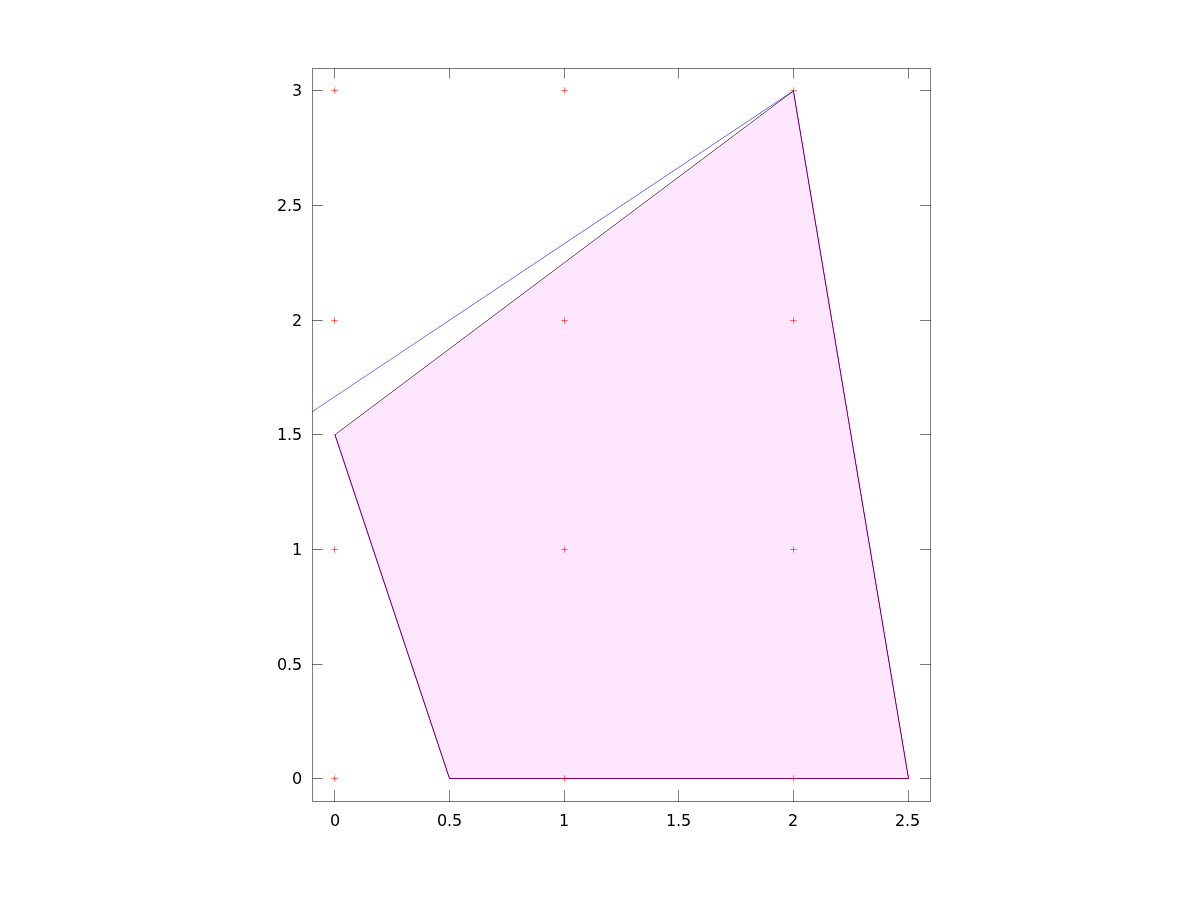
\includegraphics[width=\textwidth]{ex11_1_a_1.png}
\end{center}

  \item x
\end{enumerate}

\subsection{Lagrangean Relaxation II}

x

\subsection{Structural alignment}

x

\end{document}
